%% For double-blind review submission, w/o CCS and ACM Reference (max submission space)
\documentclass[sigplan,10pt,review]{acmart}\settopmatter{printfolios=true,printccs=false,printacmref=false}
%% For double-blind review submission, w/ CCS and ACM Reference
%\documentclass[sigplan,10pt,review,anonymous]{acmart}\settopmatter{printfolios=true}
%% For single-blind review submission, w/o CCS and ACM Reference (max submission space)
%\documentclass[sigplan,10pt,review]{acmart}\settopmatter{printfolios=true,printccs=false,printacmref=false}
%% For single-blind review submission, w/ CCS and ACM Reference
%\documentclass[sigplan,10pt,review]{acmart}\settopmatter{printfolios=true}
%% For final camera-ready submission, w/ required CCS and ACM Reference
%\documentclass[sigplan,10pt]{acmart}\settopmatter{}


%% Conference information
%% Supplied to authors by publisher for camera-ready submission;
%% use defaults for review submission.
\acmConference[PL'17]{ACM SIGPLAN Conference on Programming Languages}{January 01--03, 2017}{New York, NY, USA}
\acmYear{2017}
\acmISBN{} % \acmISBN{978-x-xxxx-xxxx-x/YY/MM}
\acmDOI{} % \acmDOI{10.1145/nnnnnnn.nnnnnnn}
\startPage{1}

%% Copyright information
%% Supplied to authors (based on authors' rights management selection;
%% see authors.acm.org) by publisher for camera-ready submission;
%% use 'none' for review submission.
\setcopyright{none}
%\setcopyright{acmcopyright}
%\setcopyright{acmlicensed}
%\setcopyright{rightsretained}
%\copyrightyear{2017}           %% If different from \acmYear

%% Bibliography style
\bibliographystyle{ACM-Reference-Format}
%% Citation style
%\citestyle{acmauthoryear}  %% For author/year citations
%\citestyle{acmnumeric}     %% For numeric citations
%\setcitestyle{nosort}      %% With 'acmnumeric', to disable automatic
                            %% sorting of references within a single citation;
                            %% e.g., \cite{Smith99,Carpenter05,Baker12}
                            %% rendered as [14,5,2] rather than [2,5,14].
%\setcitesyle{nocompress}   %% With 'acmnumeric', to disable automatic
                            %% compression of sequential references within a
                            %% single citation;
                            %% e.g., \cite{Baker12,Baker14,Baker16}
                            %% rendered as [2,3,4] rather than [2-4].


%%%%%%%%%%%%%%%%%%%%%%%%%%%%%%%%%%%%%%%%%%%%%%%%%%%%%%%%%%%%%%%%%%%%%%
%% Note: Authors migrating a paper from traditional SIGPLAN
%% proceedings format to PACMPL format must update the
%% '\documentclass' and topmatter commands above; see
%% 'acmart-pacmpl-template.tex'.
%%%%%%%%%%%%%%%%%%%%%%%%%%%%%%%%%%%%%%%%%%%%%%%%%%%%%%%%%%%%%%%%%%%%%%


%% Some recommended packages.
\usepackage{booktabs}   %% For formal tables:
                        %% http://ctan.org/pkg/booktabs
\usepackage{subcaption} %% For complex figures with subfigures/subcaptions
                        %% http://ctan.org/pkg/subcaption


\newcommand{\atl}{ATLAS }
\newcommand{\gem}{GEMM }

\begin{document}

%% Title information
\title[Short Title]{Capri-Based ATLAS: A Faster and Better Linear Algebra Auto-tunning Library}         %% [Short Title] is optional;
                                        %% when present, will be used in
                                        %% header instead of Full Title.
%% \titlenote{with title note}             %% \titlenote is optional;
                                        %% can be repeated if necessary;
                                        %% contents suppressed with 'anonymous'


%% Author information
%% Contents and number of authors suppressed with 'anonymous'.
%% Each author should be introduced by \author, followed by
%% \authornote (optional), \orcid (optional), \affiliation, and
%% \email.
%% An author may have multiple affiliations and/or emails; repeat the
%% appropriate command.
%% Many elements are not rendered, but should be provided for metadata
%% extraction tools.

%% Author with single affiliation.
\author{Yan Pei}
\affiliation{
  \department{Department of Computer Science}  %% \department is recommended
  \institution{University of Texas at Austin}  %% \institution is required
}
\email{ypei@cs.utexas.edu}          %% \email is recommended

%% Author with two affiliations and emails.
\author{Jiayuan He}
\affiliation{
  \department{Department of Computer Science}  %% \department is recommended
  \institution{University of Texas at Austin}  %% \institution is required
}
\email{hejy@cs.utexas.edu.com}         %% \email is recommended

%% Abstract
%% Note: \begin{abstract}...\end{abstract} environment must come
%% before \maketitle command
\begin{abstract}

Auto-tuning is a general approach to find the optimal optimization parameters such as tile sizes in matrix multiplication.
There are two main approaches in auto-tuning: empirical search and model-based.
Empirical search is universal but slow, and some heuristic to reduce search space may prune out best solutions.
Model-based auto-tuning predicts the best parameters by platform abstractions but the performance can degrade.
\par
ATLAS uses orthogonal line search to find optimal parameters.
The search takes a long time and the space is not guaranteed to include the optimal points.
In this project, we introduce Capri-based ATLAS search, to reduce the search time and achieve high performance simultaneously.
Capri first takes the results of exhaustive search and trains them offline. During the ATLAS code generation, it provides candidate parameters for ATLAS to run on the platform and pick the best.
\par
We evaluate the system on 12 platforms. Our experiments show that  Capri-based ATLAS search achieves XXX speedup over ATLAS orthogonal line search and it only suffers YYY performance degradation.


\cite{yotov2005search}\cite{sui2016proactive}
 \ldots.

\end{abstract}

%% 2012 ACM Computing Classification System (CSS) concepts
%% Generate at 'http://dl.acm.org/ccs/ccs.cfm'.
\begin{CCSXML}
<ccs2012>
<concept>
<concept_id>10011007.10011006.10011008</concept_id>
<concept_desc>Software and its engineering~General programming languages</concept_desc>
<concept_significance>500</concept_significance>
</concept>
<concept>
<concept_id>10003456.10003457.10003521.10003525</concept_id>
<concept_desc>Social and professional topics~History of programming languages</concept_desc>
<concept_significance>300</concept_significance>
</concept>
</ccs2012>
\end{CCSXML}

\ccsdesc[500]{Software and its engineering~General programming languages}
\ccsdesc[300]{Social and professional topics~History of programming languages}
%% End of generated code


%% Keywords
%% comma separated list
\keywords{Autotunning, Approximation, ATLAS, Capri, high performance computing,
linear Algebra, design space exploration, exhaustive search, orthogonal search,
model-based search, ,machine learning, decision tree}  %% \keywords are mandatory in final camera-ready submission


%% \maketitle
%% Note: \maketitle command must come after title commands, author
%% commands, abstract environment, Computing Classification System
%% environment and commands, and keywords command.
\maketitle


\section{Introduction}
\label{sec:intro}

A key step in program optimization is the estimation of optimal values for
parameters such as tile sizes and loop unrolling factors.
Currently programmers usually rely on optimization techiques provided by traditional compilers, which
is often too generalized to produce desired performance.
General compiler techniques cannot take care of applications such as general matrix multiply(GEMM),
whose performance is heavily based on those optimization parameters.
On the other hand, writing highly optimized code is impractical for average
programmers because it needs huge amount of prior knowledge both in application
itself and the target platform.


%Optimization parameters of high performance programs must be tuned for a given platform.
%how the program is written and how the optimization parameter is set.
\par

Auto-tuning is a straight-forward and one of the simplest way to find the optimal parameters.
There are two major category of auto-tuning approaches: empirical search and model-based tuning.
\par
Empirical search tries to find the best performing code by searching every data point in
the parameter space and evaluate the performance of them on the actual hardware.
It has been successfully applied to build a variety
of high-performance domain-specific libraries including
dense linear algebra [Clint Whaley et al., 2001, Bilmes et al.,
1997], sparse linear algebra [Vuduc et al., 2005], signal processing
[Frigo and Johnson, 2005], sorting [Li et al., 2004],
general stencil operations [Kamil et al., 2010], etc.
\par
However, exaustively searching the whole parameter space is slow and impractical.
The search space is usually too large for modern machines and contains lots of low performance points where
searching is unnecessary. Consequently, most proposed searching methods
prune the space with hard-coded heuristics and may lose generality on new platforms.

\par
The second approach of auto-tuning is model-based tuning, which builds an analytical model
to estimates optimal parameters. The significant advantage of such approach is fast. Good optimization
parameters can be directly derived from the analytical model.
However in practice, it is generally difficult to build a highly accurate analytical model bacause of the growing complexity
of modern architectures and applications. The analytical model is inflexible and has to be built by expert of both architecture
and application.

\par
To address this weakness, it is intuitive to combine the two approaches together by first pruning the search
space with an automatically generated model, and then evaluate candidates
provided by the model to get the best set of parameters.
On the other hand, the time taken to generate an optimized set of parameters
should also be taken into consideration. In some cases, users are not willing
to wait for a day or two, or even an hour to get the most optimized result, an
``enough good'' result is usually ok. Therefore, approximation can be introduced
to accelerate the optimization process.

There is growing interest in approximate computing as a way of reducing energy
and time required to execute applications. \cite{ansel2011language,
baek2010green, sidiroglou2011managing, swaminathan2015case}. In conventional
computing, programs are usually treated as implementations of mathematical
fuctions, so there is a precise output that must computed for a given input.
However, in many problem domains, it is sufficient to produce an ``enough''
good result: for example, when rendering a image in graphics, it is
acceptable to take computational short-cuts if the graph doesn't hurt user's
experience. In addition, since analytical models are often imprecise for
applicatons with high complexity. Machine learning models can be a great
subsitute. In this paper, we use Capri\cite{sui2016proactive}, a published
approximate program, to build machine learning based models for \gem performance
based on different parameter settings. We denote parameter settings as knobs in
our paper.

The contributions of this papers are:
1.
2.
3.

\par
The rest of this paper is organized as follows. Section [motivation and background] describes the details of ATLAS
orthogonal line search and Capri system.
Section [Design] introduces the implementation of Capri-based ATLAS search.
Section [Experiment Methodology] provides the details of experiment methodology.
Section [results] shows all the results of our system, analyze and compare them with ATLAS orthogonal search.
Section [related work] provides an overview of related work.
And finally, section [conclusion] concldes and outlines our possible future work.

\section{Background}
\label{sec:background}

  \subsection{ATLAS code generator}
  \label{sec:atlas_intro}
  ATLAS uses orthogonal line search to auto-tune its optimization parameters.
  It assumes that the parameters are independent to performance and the optimal values can be
  restricted by some architecture features like number of registers, size of L1 cache.
  Even though ATLAS empirical can generate good parameters, its search space is still not guaranteed to contain
  the optimal point, and there are still many low performance points in the search space which is unnecessary
  to search.

  \subsection{Capri approximation program}
  \label{sec:Capri_intro}
  a

\section{Motivation}
\label{sec:moti}

\section{Design}
\label{sec:design}

\section{Experiment Methodology}
\label{sec:experiment}

In the experiment, we only consider single precision, real number matrix multiplication. We implement 
an exhaustive search on ATLAS. The space of each parameter in $NB$, $MU$, $NU$, $KU$ are not smaller 
than the ATLAS orthogonal search, and the exhaustive search tries every possible combination of them. 
On a typical platform as we mentioned in Section \ref{atlas_intro}, it takes more than 10 hours to finish 
the search on 12960 points. 



\section{Evaluation}
\label{sec:evaluation}

  \subsection{Exhaustive search vs \atl orthogonal search}
  \label{sec:exhaustiveVSorthogonal}
  \begin{figure*}[tbhp]
    \centering
    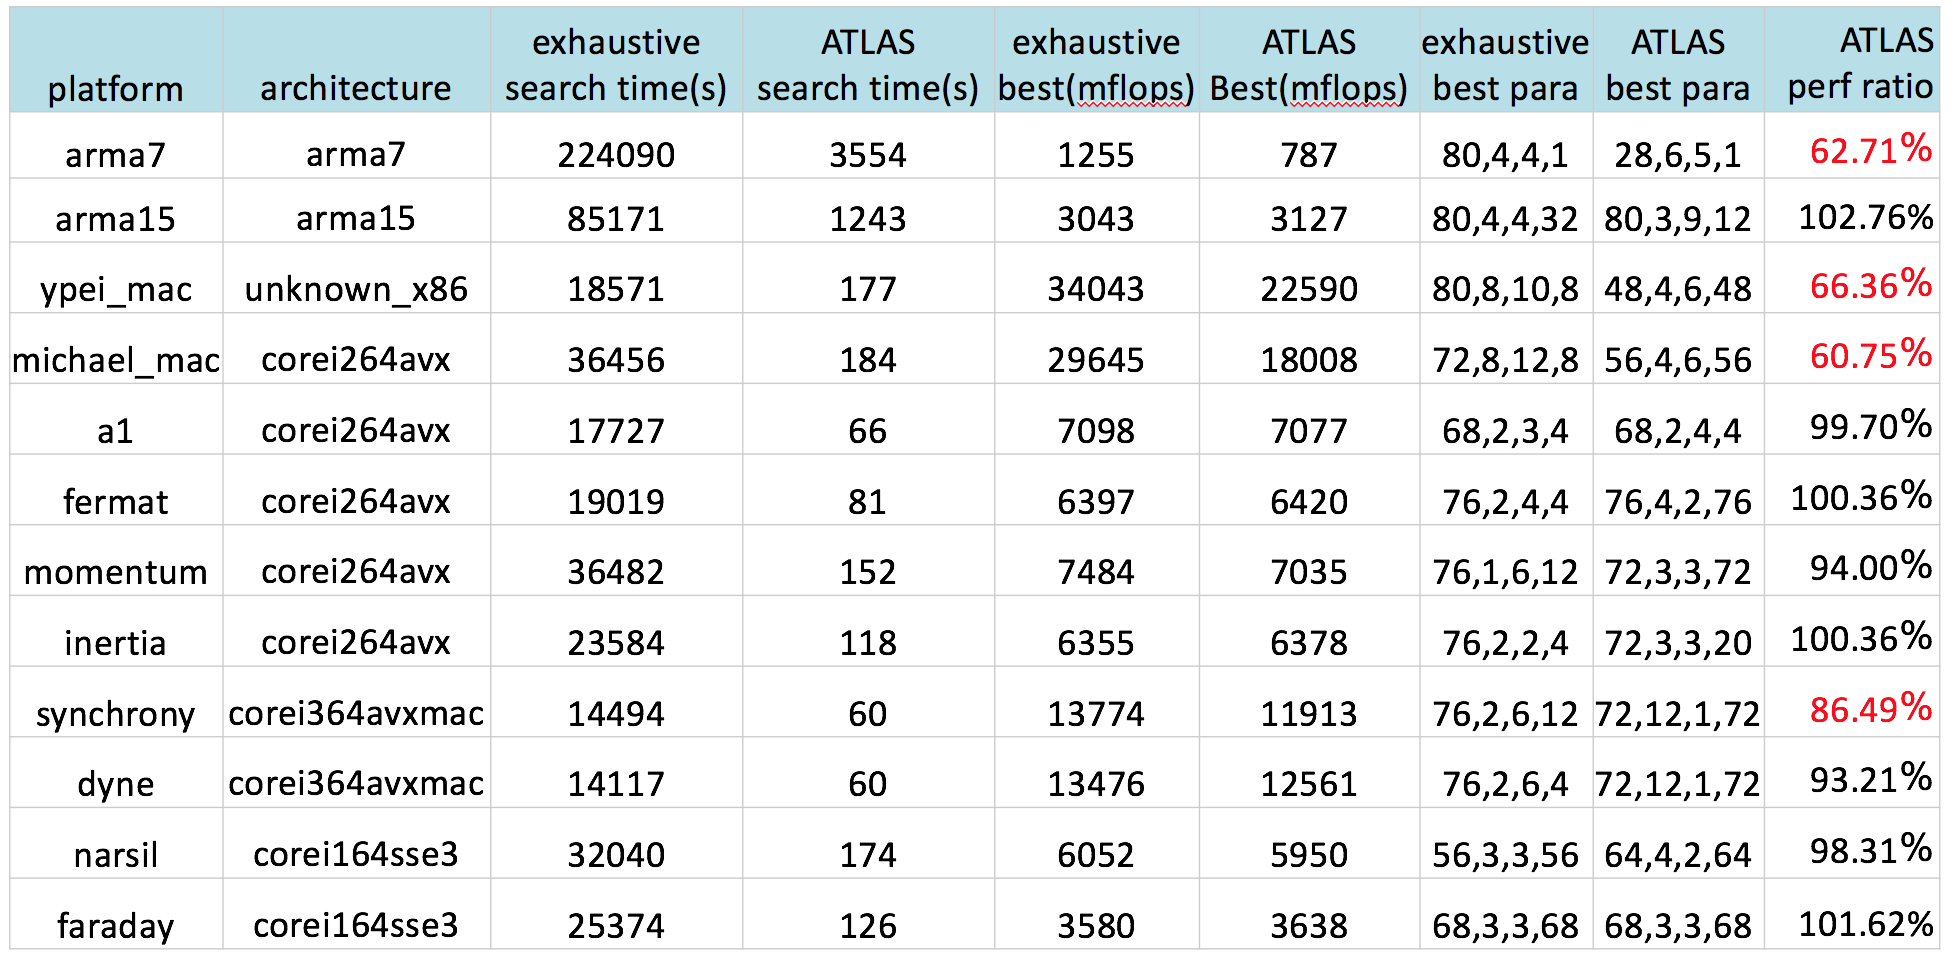
\includegraphics[width=0.9\textwidth]{images/exhaustiveVsorthogonal.png}
    \caption{Searching time comparison between exhaustive search and \atl orthogonal search}
    \label{fig:exhaustiveVsorthogonal}
  \end{figure*}
  In this section, we compare the result of \atl orthogonal search with the best of exhaustive
  search. The search time, generated code performance, and selected parameters are listed in Figure
  \ref{fig:exhaustiveVsorthogonal}.\par
  Except for the two ARM processors, it takes around one to three minutes for ATLAS orthogonal search
  to generate its best code. Considering that we only search for single precision, real number general
  matrix multiplication, we haven't run double precision, complext number or some other benchmarks
  like transpose matrix kernel, matrix vector kernel, big matrix kernel, rank-1 matrix kernel etc, installing
  ATLAS may take hours to finish. The orthogonal search is still too slow to end user.\par
  Column \textit{exhaustive best} and \textit{ATLAS best} list the FMLOPS performance of generated code from
  both search strategy. The ratio of ATLAS over exhaustive is in the last column. On 8 platforms,
  ATLAS is able to generate code with >90\% of best performance. Three platforms has only around 60\% of
  best performance. The two parameter columns list the selected paraeters in the order of $(NB, MU, NU, KU)$.\par
  Note for the two MAC platform that, the two middle parameters (MU, NU) are so large that it exceeds
  the register requirement of \[ MU*NU + MU + NU + LS < NR \]. Thus ATLAS orthogonal search is not able
  to find it. Currently we do not have a clear explanation to this. One guess is that, the CORE i7 processors
  have more physical registers than ISA architecture register. The ISA is only able to use or identify 32 registers.
  However due to register renaming, it can make use of more than 32 registers and the extra registers are not visible
  to softwares.\par

  \subsection{GEMM performance model}
  \label{sec:GEMMperf}
  This section discuss whether it is easy to build a model of \gem performance
  given platform information and a knob setting. Intuitively, we evaluate
  whether the \gem performance is predictable. In Fig.\ref{fig:inertia_perf},
  we shows the performance prediction accuracy on platform inertia using a model
  trained by M5 on the other 11 platforms. Each point represent one knob
  setting. This figure shows the comparison between the normalized actual
  performance and the predicted performance. There are two views to evaluate
  this figure. The first view is to see the distance between the points to the
  $y=x$ line. The distance evaluates how accurate the model is.

  Another point of
  view is to focus on the few highest data points, which are the points in the
  red oval in Fig.\ref{fig:inertia_perf}. These points represent the highest
  predicted performance, which will be selected as the candidate knob settings
  in \atl evaluation. The corresponding x axis value is the actual performance
  number for this knob setting. Intuitively, the lefter the point is, the
  better the prediction is, we want high prediction to indicate high actual
  performance. Note that only the knob settings with high performance are
  interested, so the prediction accuracy for low points doesn't matter much in
  this case as soon as high prediction point are left enough.

  Inertia is doing well in both of the views, while platforms like arma7 is not
  because it's really hard to use data collected from 10 Intel processors and 1
  ARM processor to predict another ARM processor's performance, as shown in
  Fig.\ref{fig:arm_perf}. The overall performance prediction, shown in
  Fig.\ref{fig:overall_perf}, is generated by randomly selecting 80\% and 20 \%
  of the data set formed by 12 platforms as training data and testing data
  respectively. It shows the overall difficulty of modeling \gem performance
  is not hard.

  \begin{figure}[bhp]
    \centering
    \begin{subfigure}[b]{1.0\linewidth}
      \centering
      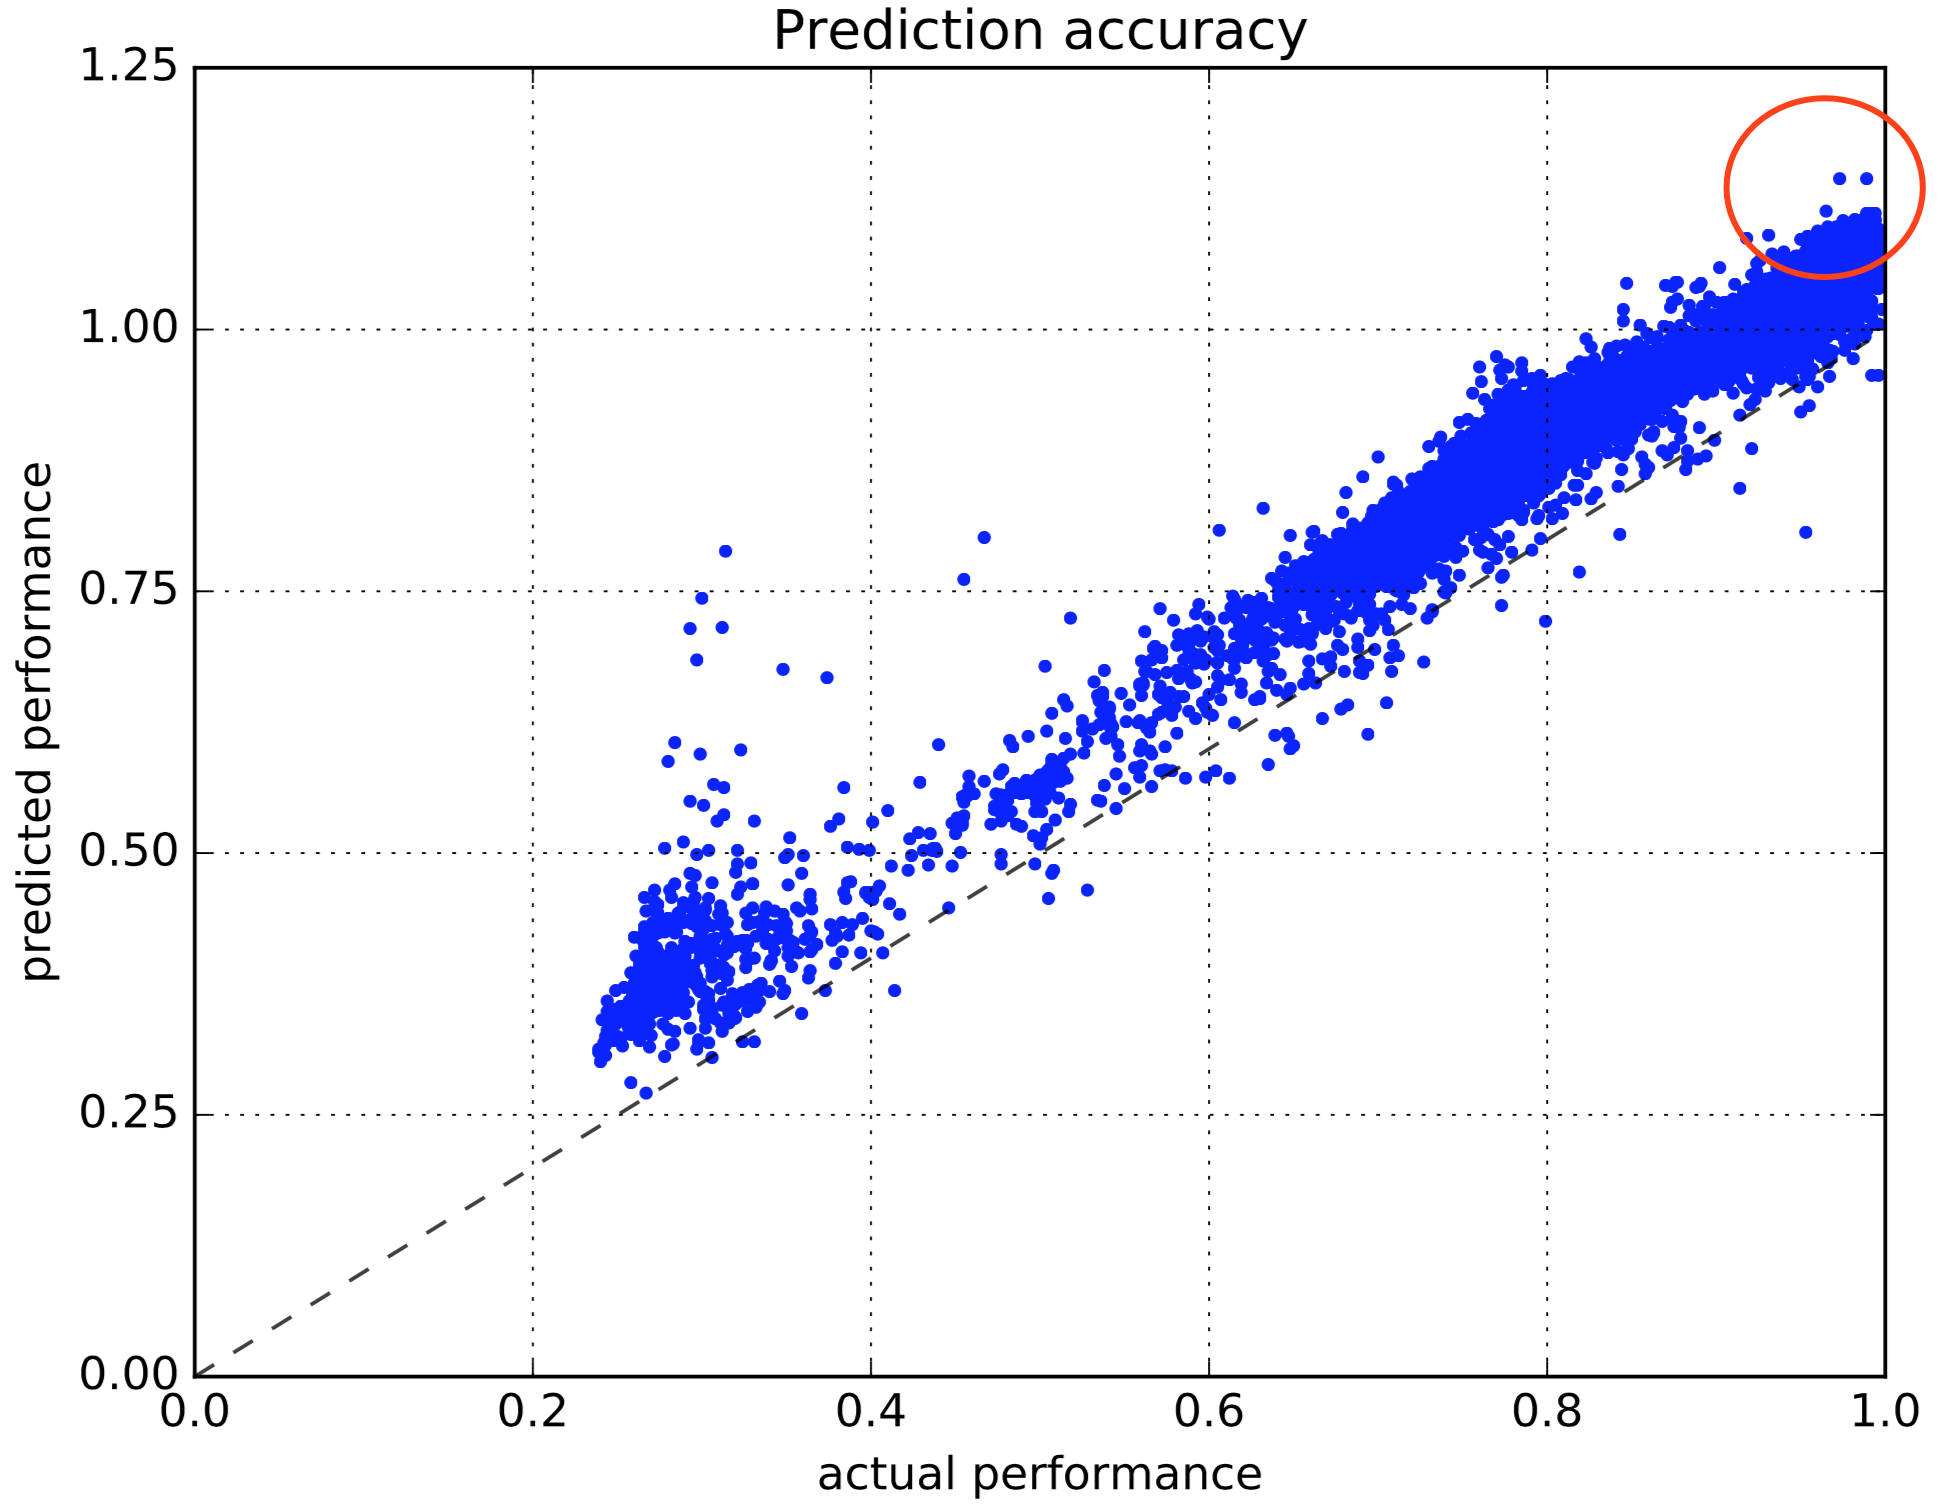
\includegraphics[width=0.8\textwidth]{images/inertia_perf.png}
      \caption{Inertia performance prediction}
      \label{fig:inertia_perf}
    \end{subfigure}
    \begin{subfigure}[b]{1.0\linewidth}
      \centering
      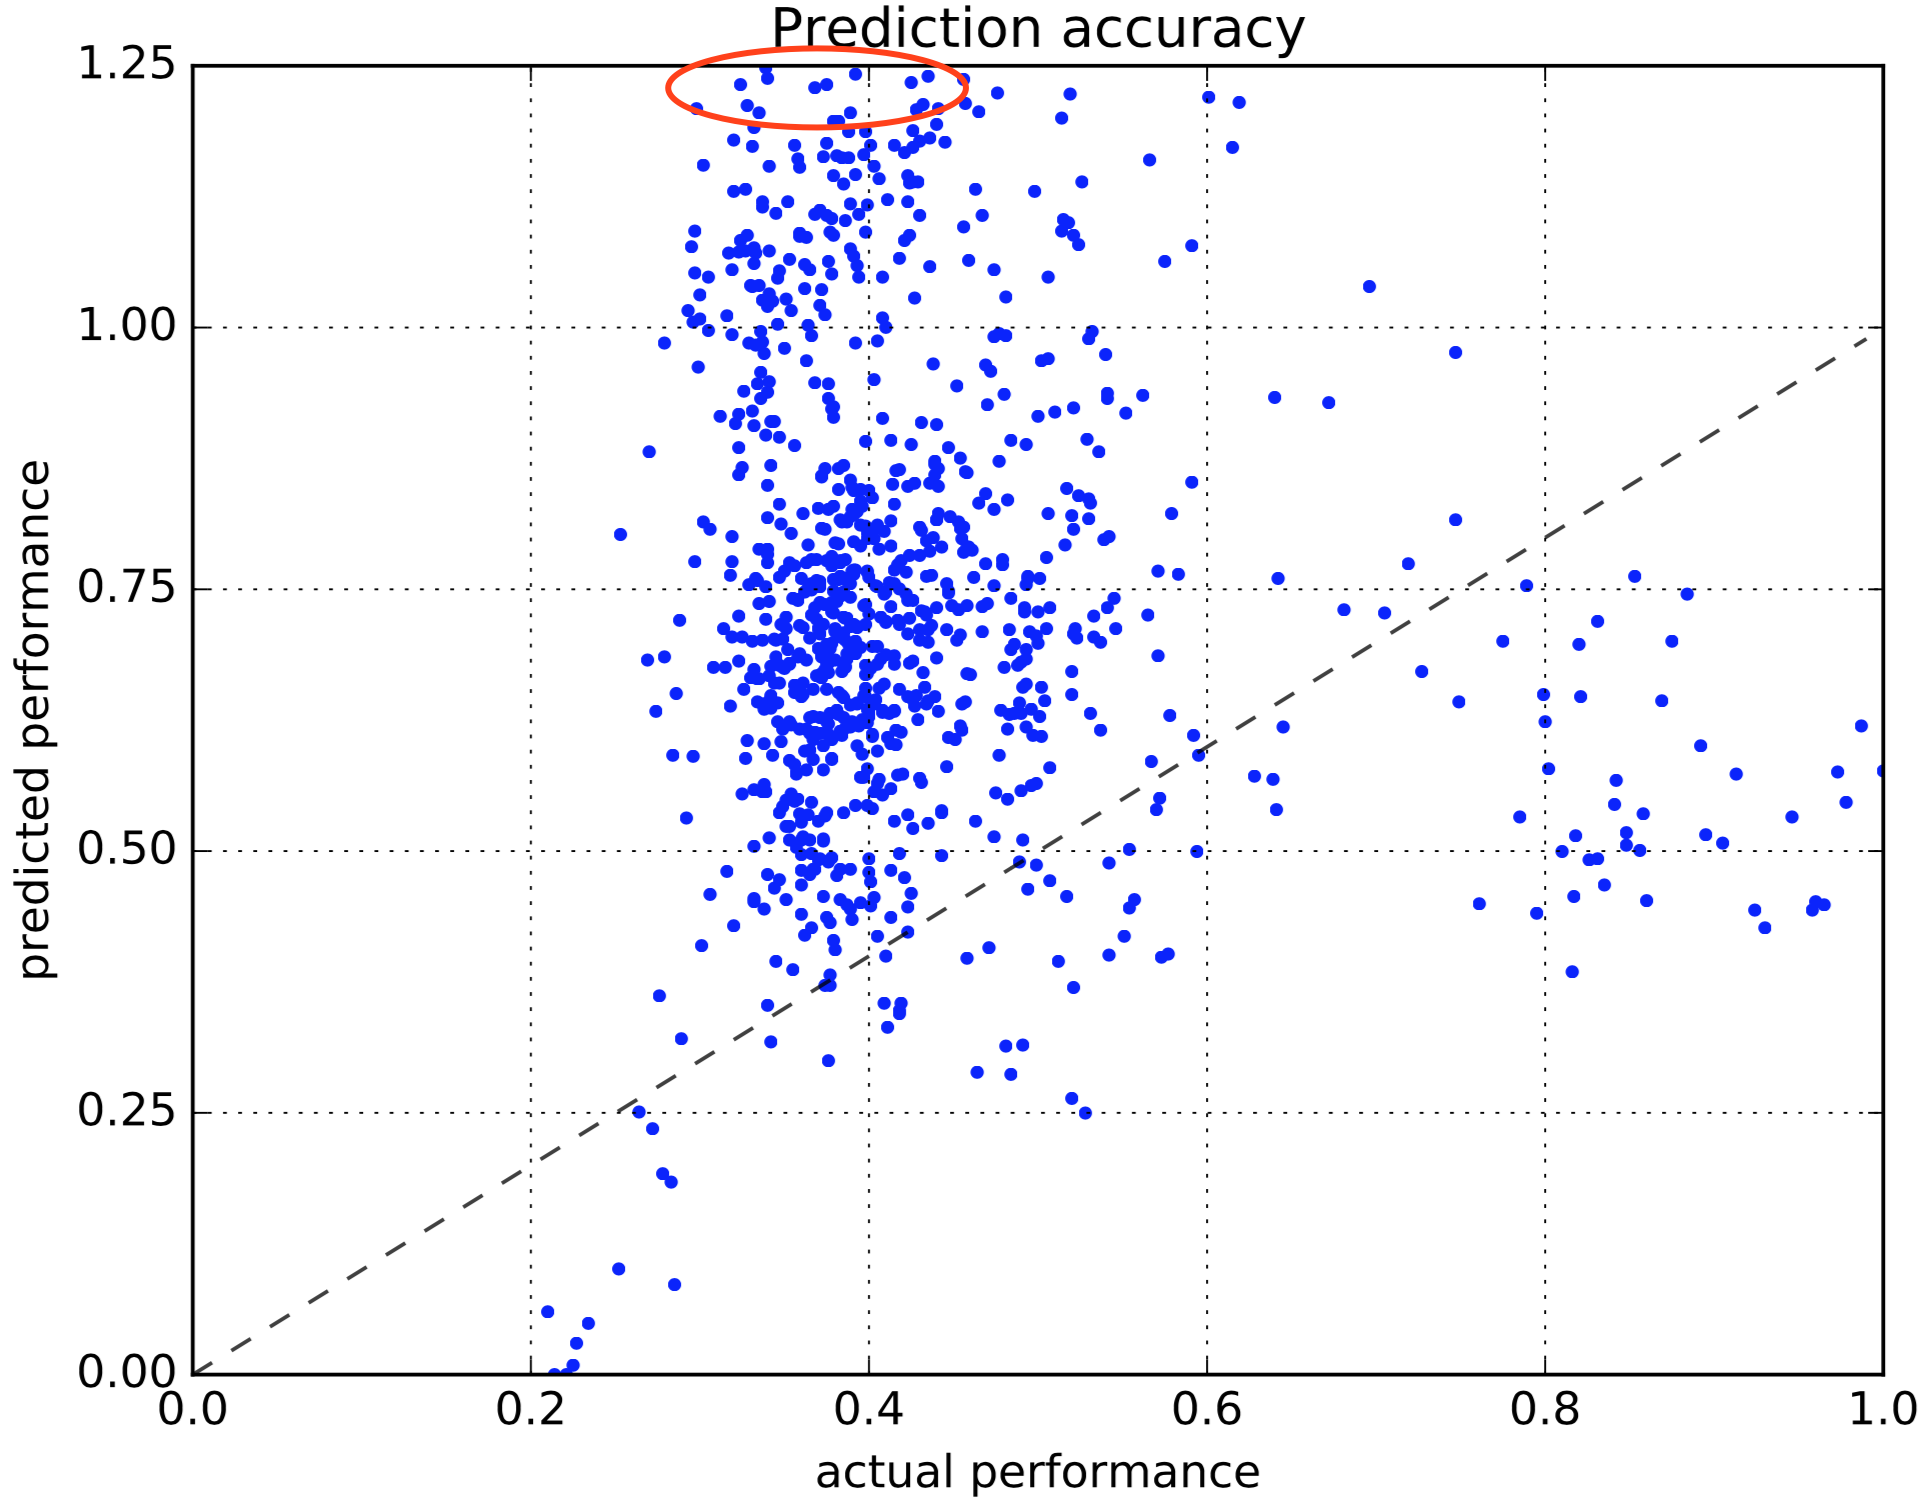
\includegraphics[width=0.8\textwidth]{images/arm_perf.png}
      \caption{Arma7 performance prediction}
      \label{fig:arm_perf}
    \end{subfigure}
    \begin{subfigure}[b]{1.0\linewidth}
      \centering
      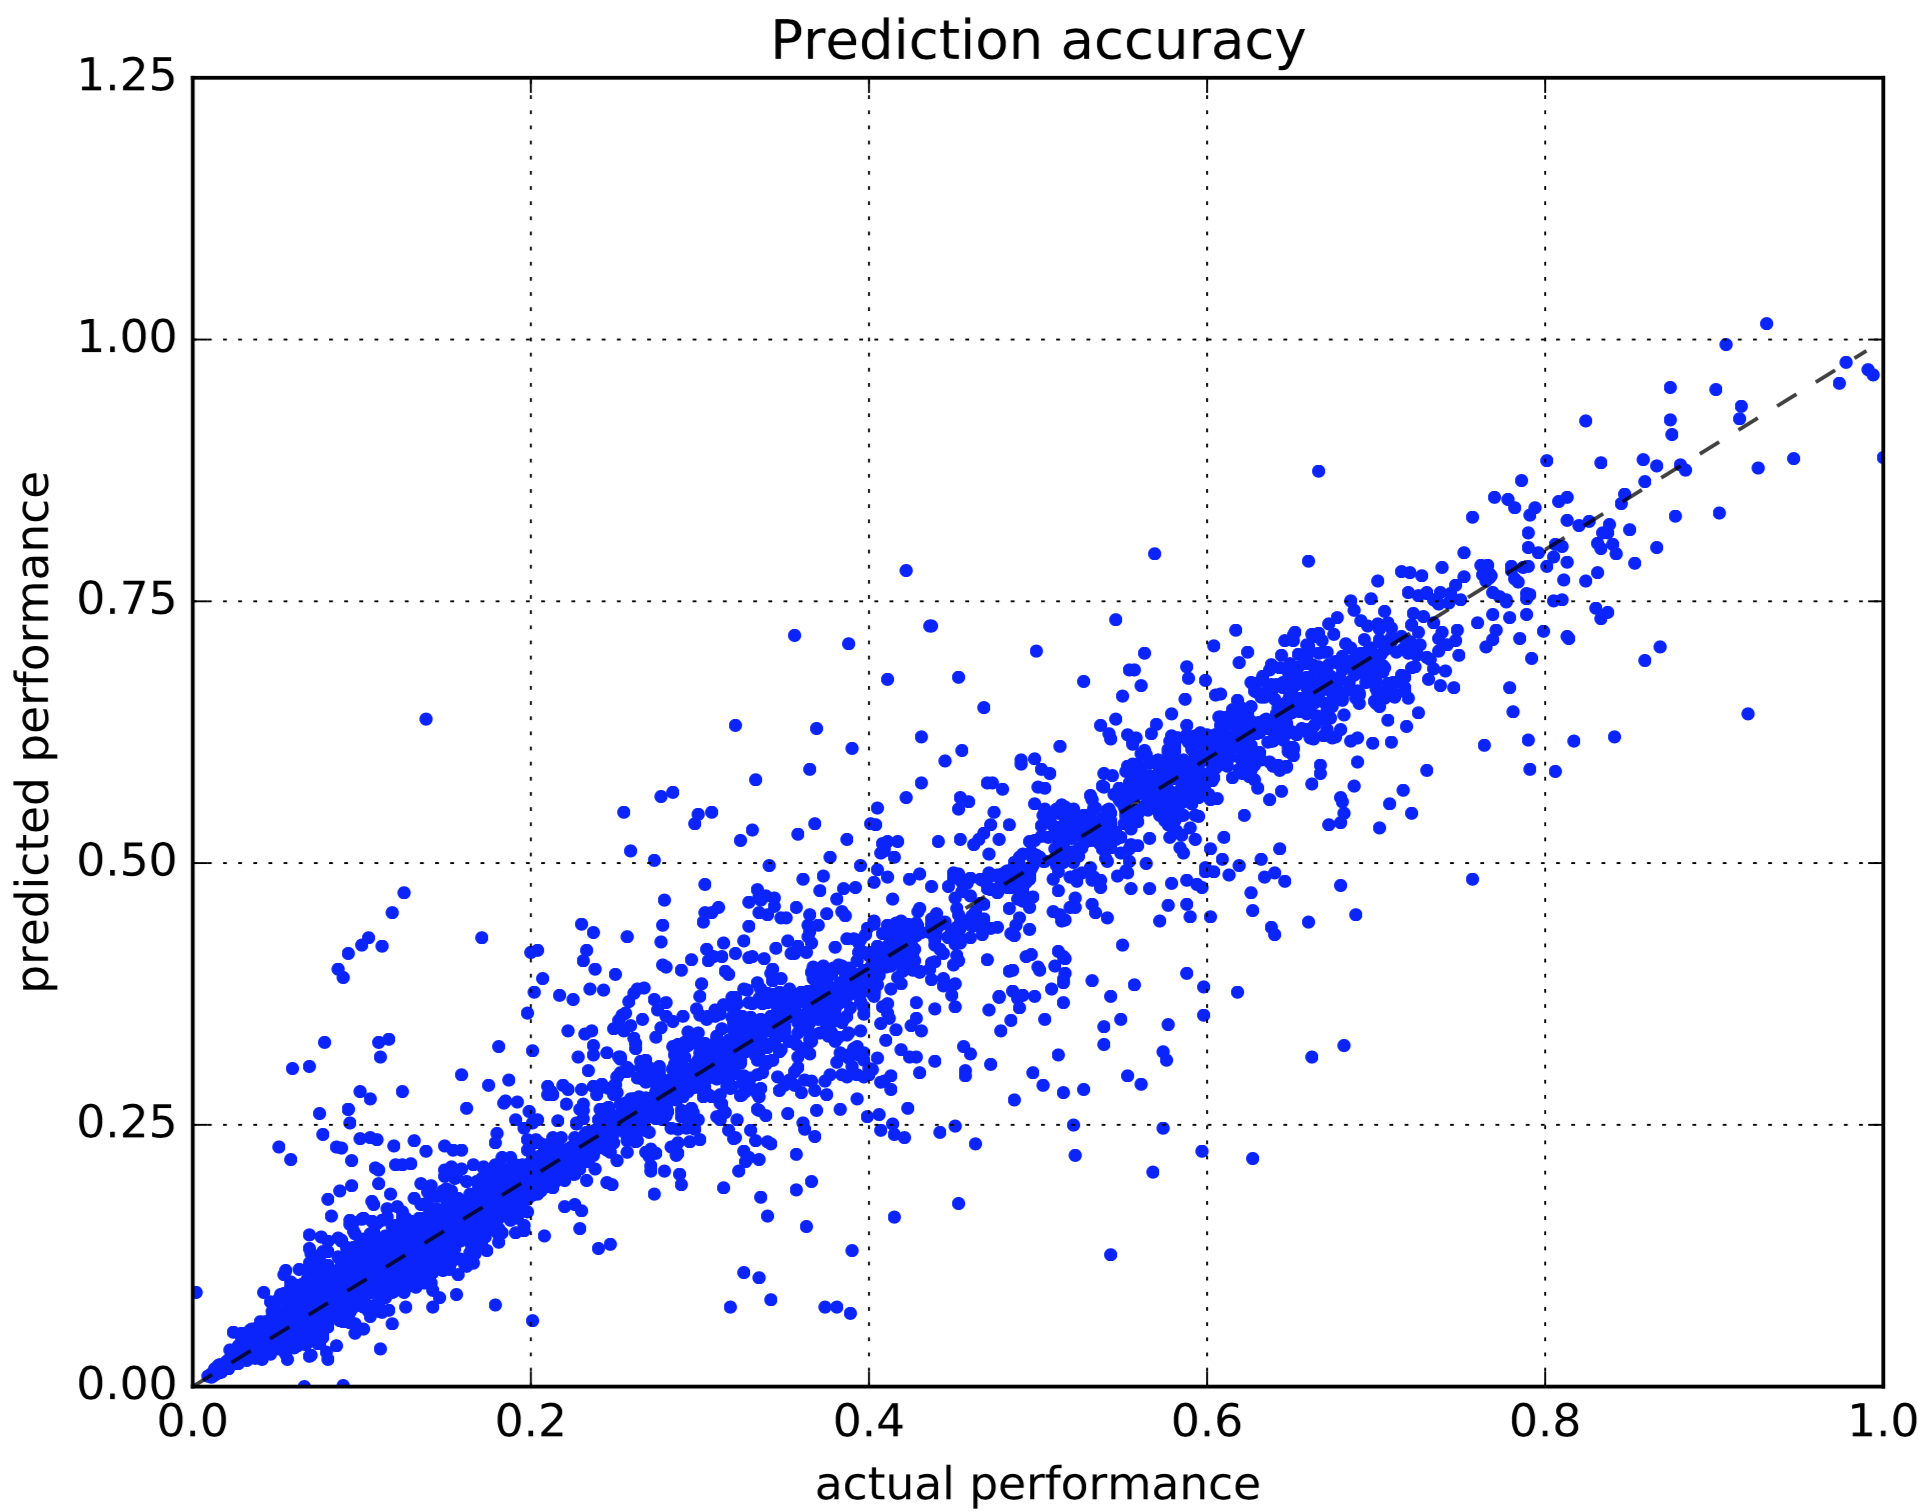
\includegraphics[width=0.8\textwidth]{images/overall_model.png}
      \caption{Overall performance prediction}
      \label{fig:overall_pref}
    \end{subfigure}
  \end{figure}


  
  \subsection{Capri-based ATLAS searching time}
  \label{sec:capri_atlas_searching}
  In this section we compare one of our evaluation metric: searching time. An overview of the result is listed in
  Figure \ref{fig:search_time}. The \textit{ATLAS search time} column is the same as in Figure \ref{fig:exhaustiveVsorthogonal}.
  \textit{Capri search time} shows the time Capri takes to purely generate top candidates without running them. 
  \textit{Capri runtime per candicates} is the average time of each candidate running on the actual platform.
  Therefore, total Capri-based ATLAS search time which is the sum of \textit{Capri search time} and actual platform time of the candidates,
  highly depends on how many candidates that the user wants. The last two columns show the speedup over ATLAS when users pick
  10 or 5 candidates. On average, Capri-based search outperforms ATLAS orthogonal search by \textbf{10.88X} on 10 candidates and \textbf{17.97X} on 
  5 candidates. On the two ARM platforms, Capri-based search can even reach more than 200X speedup.
  


  \begin{figure*}[tbhp]
    \centering
    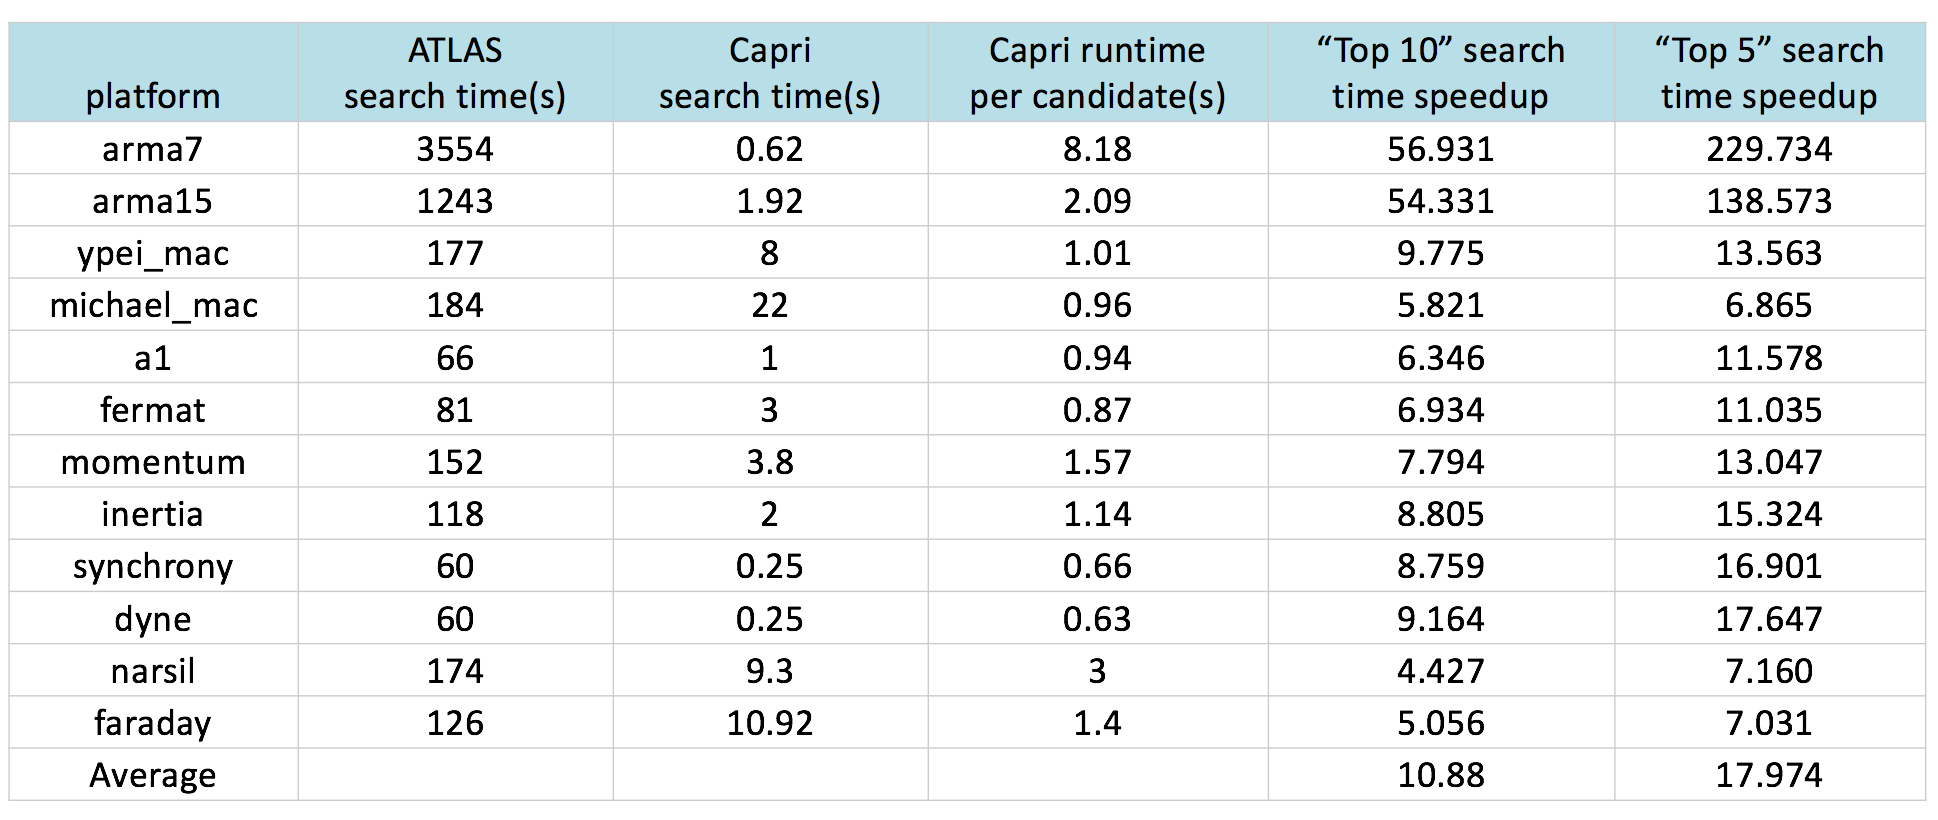
\includegraphics[width=0.9\textwidth]{images/timespeedup.png}
    \caption{Capri-based ATLAS searching time speedup}
    \label{fig:search_time}
  \end{figure*}

  \subsection{Capri-based ATLAS performance}
  \label{sec:capri_atlas_performance}

  \begin{figure*}[tbhp]
    \centering
    \begin{subfigure}[b]{1.0\linewidth}
      \centering
      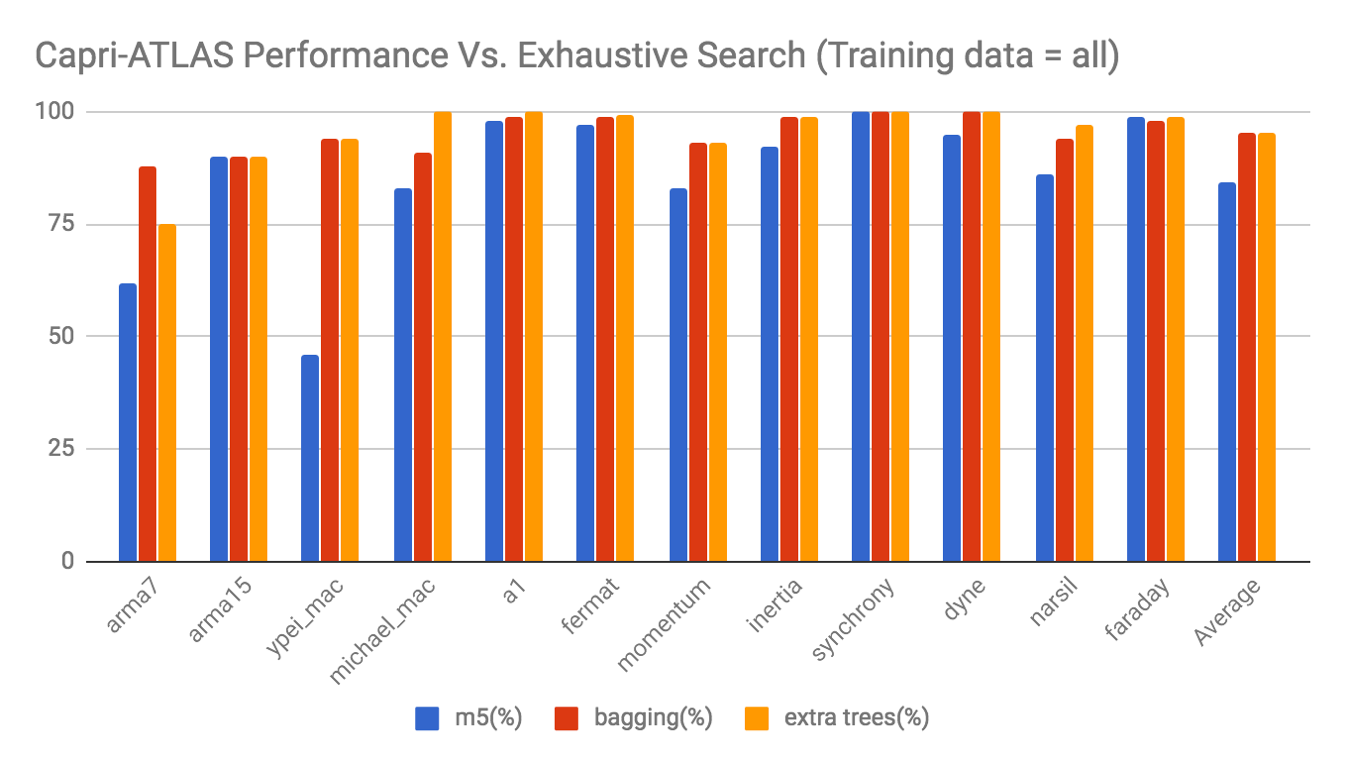
\includegraphics[width=0.85\textwidth]{images/all_perf.png}
      \caption{ }
      \label{fig:all_perf}
    \end{subfigure}
    \begin{subfigure}[b]{1.0\linewidth}
      \centering
      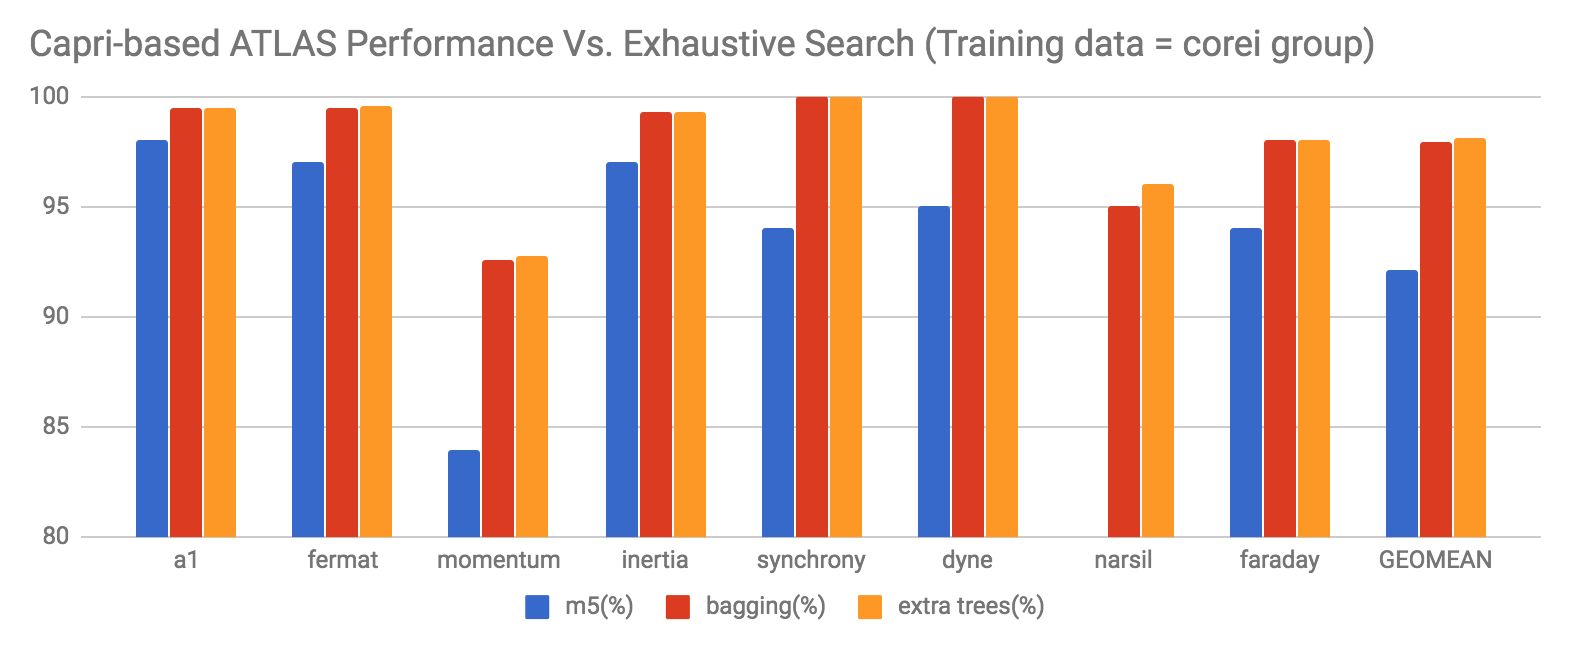
\includegraphics[width=0.85\textwidth]{images/corei_perf.png}
      \caption{ }
      \label{fig:corei_perf}
    \end{subfigure}
    \begin{subfigure}[b]{1.0\linewidth}
      \centering
      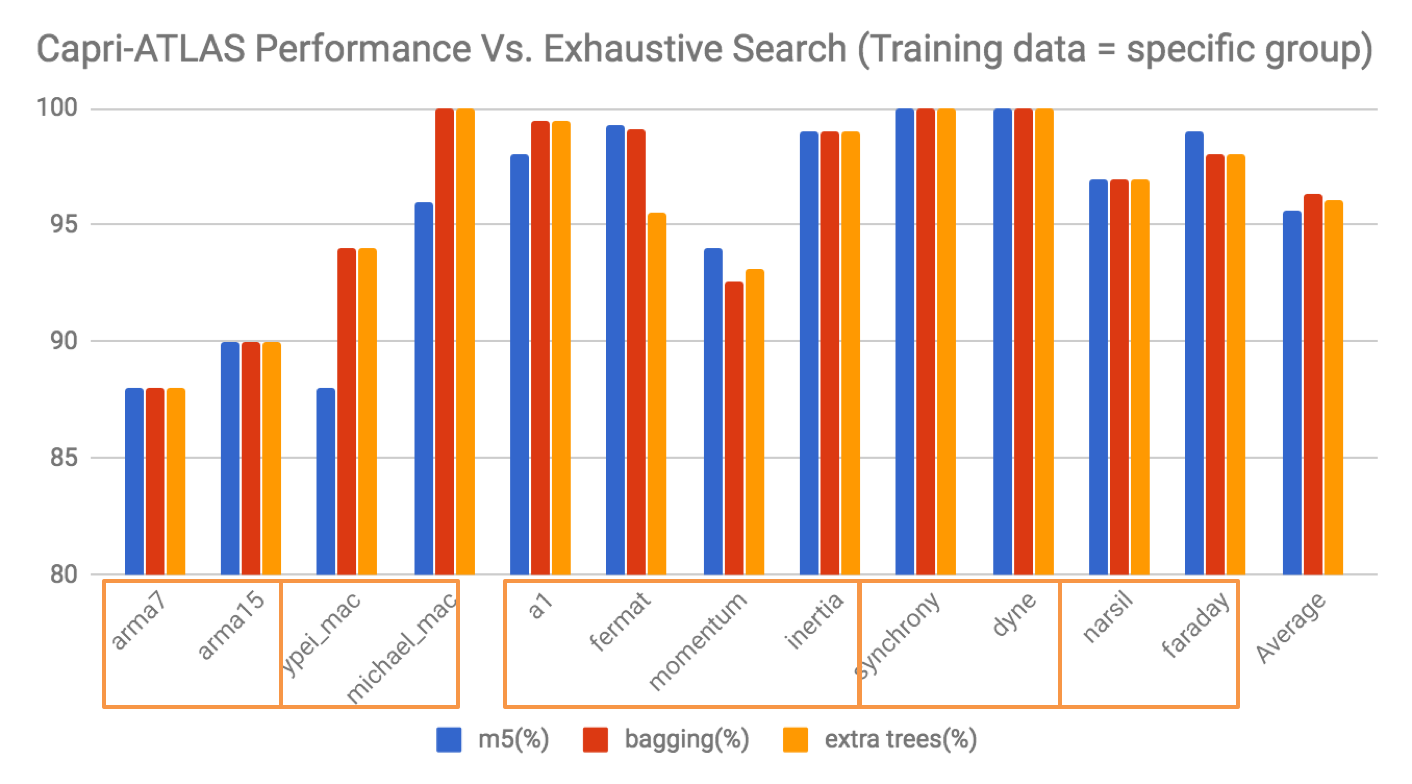
\includegraphics[width=0.85\textwidth]{images/specific_perf.png}
      \caption{ }
      \label{fig:specific_perf}
    \end{subfigure}
  \caption{Capri-based \atl Performance using different training sets}
  \end{figure*}

  \subsection{Parameter sensitivity}
  \label{sec:parametersensitivity}
  \begin{figure*}[tbhp]
    \centering
    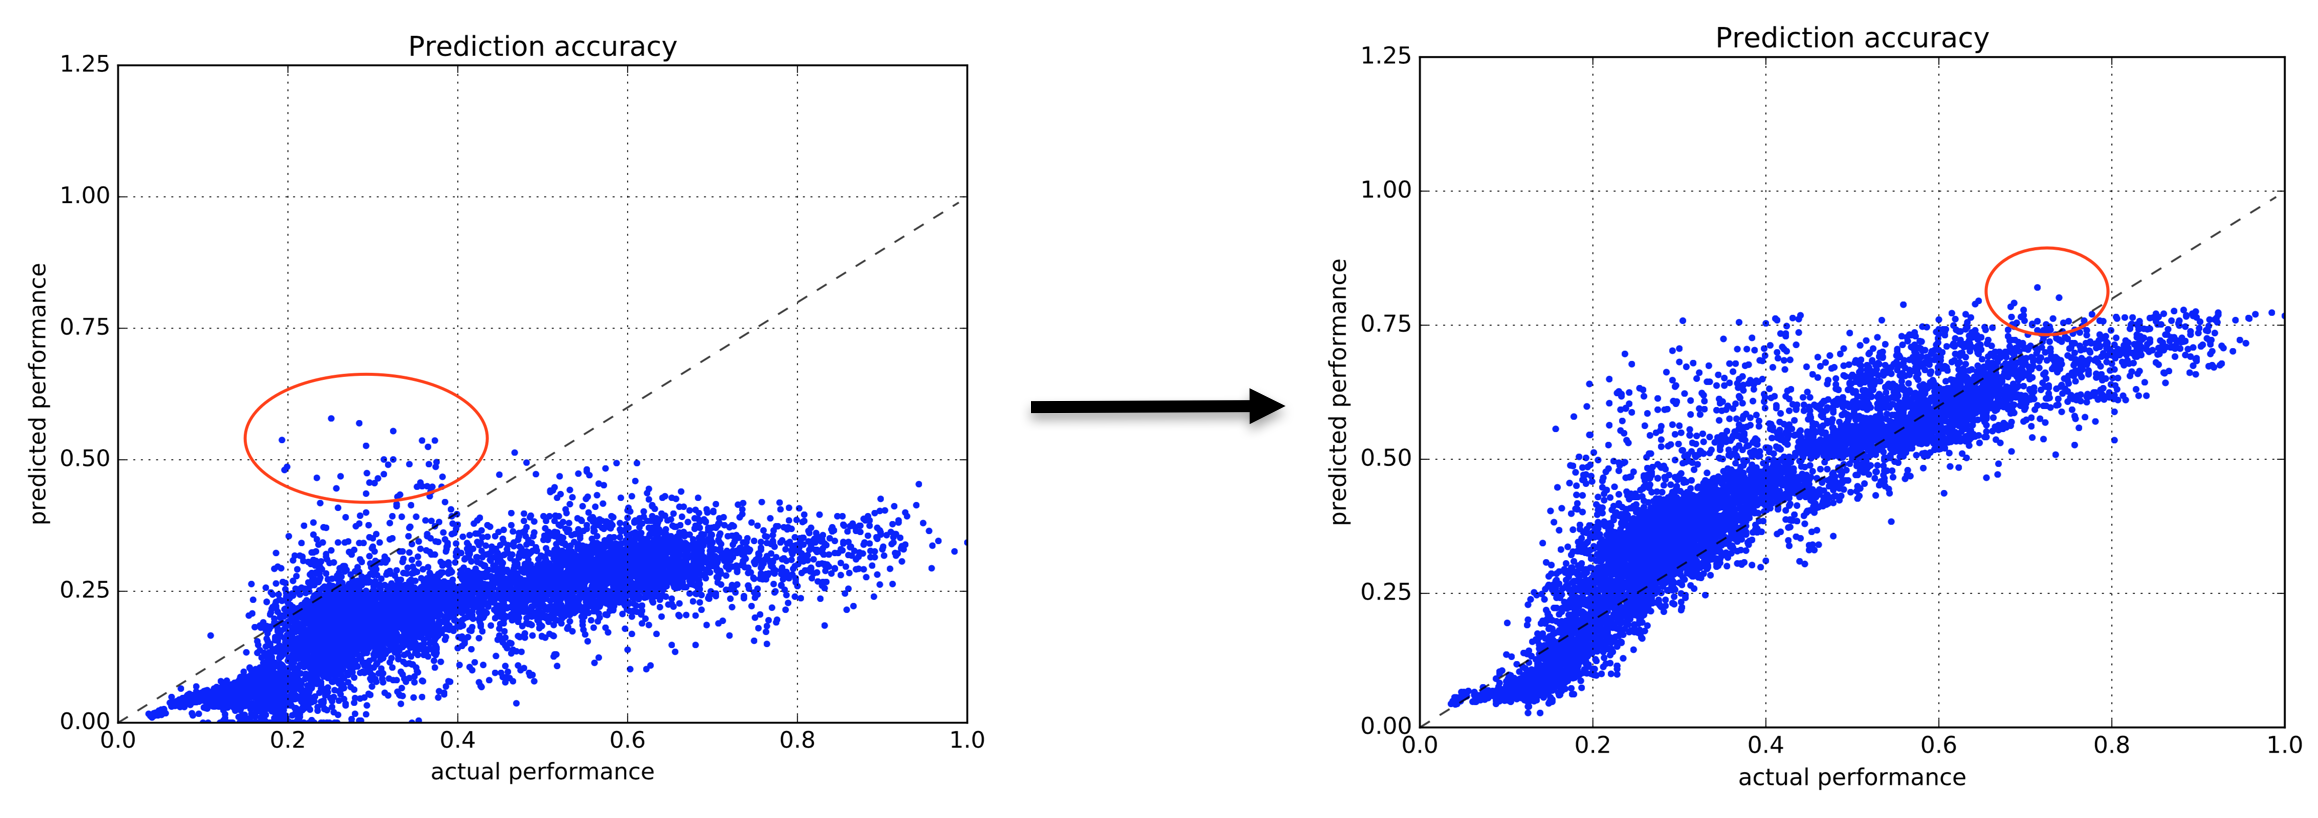
\includegraphics[width=0.9\textwidth]{images/ypei_perf_change.png}
    \caption{Performance improves when a better training set is selected}
    \label{fig:ypei_perf_change}
  \end{figure*}

    \subsubsection{Training set}
    \label{sec:training_set}

    \subsubsection{Top M constraint}
    \label{sec:top_m}

\section{Related Work}
\label{sec:related}

There are many heuristics on pruning the searching space and improving performance of auto-tuning.

ATLAS\cite{yotov2005search} uses orthogonal to reduce the search space. It assumes that 
the optimization parameters are independent to each other and they are restricted by some hardware features.
However as we have seen in the experiment, the assumption is not always true and its generated code
may have low performance. A similar technique \cite{li2009note} is later implemented on GPU to keep up
with rapid change in hardware. FFTW\cite{frigo2005design} adopts dynamic programming where program of large size problem
is constructed from previously generated code for small size. The inherent assumption of dynamic programming is that,
the best code of a transform is independent of the calling context. This assumption holds for the arithmetic cost (which implies
that DP produces the optimal solution), but not for the runtime of transform algorithms.
SPIRAL\cite{puschel2005spiral} not only adopts dynamic programs,
but also tries exhaustive search, random search, evolutionary search and hill climbing heuristic. The property 
of evolutionary search and hill climbing makes the generated solution may be local optimal. \par

Model-driven auto-tuning is another approach. ATLAS\cite{yotov2005search} adops a model from a heuristic based on
hardware parameters. SPIRAL\cite{puschel2005spiral} build and learn a model from the features a nodes in the divide-and-conquer tree.
The feature must be carefully selected and the built model shows 10\% to 20\% performance loss. \par

It requires expertise on both hardware architectures and applications to build an accurate model. Therefore a lot of 
effort has been spent in using machine-learning to automatically learn a model. Li et al.\cite{li2004dynamically} apply machine learning 
technique to build a model for sorting. The machine learning technique predicts the best algorithm as a function of the 
characteristics of the input data set and the performance of the difference algorithms on the target platform. Falch et al.\cite{falch2015machine}
focuses on OpenCL which targets on heterogeneous system and often suffers from performance portability. They run on a random
subset of the entire tuning parameter space, and the results are used to build an artificial neural network based model. 
The model can be used to find interesting parts of the parameter space for further search. Yigitbasi et al.\cite{yigitbasi2013towards} focus on MapReduce.
They selected support vector regression model(SVR) as the most accurate machine learning model among several candidates, by 
training them with diverse MapReduce applications and cluster configurations. Bergstra et al.\cite{bergstra2012machine} build a machine learning model
with boosted regression tree and generate high performance library on multicore GPU platforms.





\section{Conclusion}
\label{sec:conclusion}



%% Acknowledgments
\begin{acks}                            %% acks environment is optional
                                        %% contents suppressed with 'anonymous'
  %% extraction tools.
  This work is based on ATLAS software and Capri project. The authors would
  like to thank Swarnendu(UTCS), Xin Sui(Tableau Software) and all the ATLAS
  developers.

  Yan Pei: I really enjoy this class. The course proves again that reading
  paper with discussion is be a great method of learning. I learned a lot
  during this class. The abstractions and high level ideas introduced in
  this class should be useful in my research career. On the other hand, I
  really wanna express my gratitude to Dr. Pingali and all my classmates.
  Thank you for preparing classes and presentations for us.

  Jiayuan He: I read a lot of papers from different areas in program synthesis, starting 
  from synthesis with algorithmic specification, to sketch, to input-output examples, to 
  natural language. I like the sketch part best, which connect incomplete programs
  with SAT solving. I learned skills to abstract high level ideas and think critically, f
  rom the presentations, summaries and discussion. Thanks Dr. Pingali and all the class 
  for the preparation and participation.
  

\end{acks}

%% Bibliography

\bibliography{reference}

%\bibliography{bibfile}




%% Appendix
\appendix
\section{Appendix}

Text of appendix \ldots

\end{document}
